\documentclass[12pt]{report}   % you have 10pt, 11pt, or 12pt options

\setlength{\textwidth}{17.2cm}     % if you change this, consider changing
\setlength{\evensidemargin}{-.3cm} % side margins to retain centering
\setlength{\oddsidemargin}{-.3cm}

\setlength{\textheight}{23cm}   % if you change this, consider changing
\setlength{\topmargin}{-2cm}  % top margin to retain centering
\setlength{\headsep}{1.6cm}

%---------------------- These packages below add functionality to your version
%of LaTeX -------------- ---------------------- You might not use all of them
%--------------------------------------
\usepackage[utf8]{inputenc}
\usepackage[T1]{fontenc}
\usepackage[]{minted}
%\usepackage[fancyvrb=true]{listings}
\usepackage{tcolorbox}
\usepackage{etoolbox}
\BeforeBeginEnvironment {minted} { \begin{tcolorbox} } 
\AfterEndEnvironment {minted} { \end{tcolorbox} }%
\usepackage{amssymb}
\usepackage{latexsym}
\usepackage{amsthm}
\usepackage{enumerate}
\usepackage{epsfig}
\usepackage{graphicx,caption,subcaption}
\usepackage{color}
\usepackage{float}
%\usepackage{hypcap}
\usepackage{amsmath}
\usepackage{makeidx}
\usepackage{fancyhdr}
\pagestyle{fancy}
\usepackage{lastpage}
\usepackage{url}
\usepackage{algorithm}
\usepackage{algorithmic}
\usepackage[algo2e]{algorithm2e}
\usepackage{appendix}
\usepackage{bm}
\usepackage{lmodern} % load a font with all the characters
\usepackage[square, numbers, comma, sort&compress]{natbib}
%------------------------- Customized Header
%--------------------------------------------------------
\fancyhead{}
\fancyfoot{}			
\lhead{Stereo Camera + IMU/INS + GPS}
\rhead{Page \thepage\ of \pageref{LastPage}}

%---------- the symbols below will give you the blackboard bold of R, T, etc.
%----------
\DeclareSymbolFont{AMSb}{U}{msb}{m}{n}
\DeclareMathSymbol{\Sph}{\mathbin}{AMSb}{"53}
\DeclareMathSymbol{\R}{\mathbin}{AMSb}{"52}
\DeclareMathSymbol{\T}{\mathbin}{AMSb}{"54}
\DeclareMathSymbol{\Z}{\mathbin}{AMSb}{"5A}
\DeclareMathSymbol{\K}{\mathbin}{AMSb}{"4B}

%------------------------- Theorem and Proof Environments
%-------------------------------------------------

% This section defines all the environments you might use.  Just type
% \begin{theorem, or corollary, or whatever}, then the optional name of the
% theorem inside {} (or empty {} if no name), then body of the theorem,
% corollary, whatever, also inside {} then \end{theorem, corollary, whatever}
%
% Notice when I use them in the paper, I put an optional "argument" to the
% function and this gives a name to the theorem

\newenvironment{theorem}[1]{\vspace{.9cm}\noindent    {\bf Theorem {#1}}}{\vspace{.1cm}}
\newenvironment{lemma}[1]{\vspace{.9cm}\noindent    {\bf Lemma {#1}}}{\vspace{.1cm}}
\newenvironment{corollary}[1]{\vspace{.9cm}\noindent    {\bf Corollary {#1}}}{\vspace{.1cm}}
\newenvironment{definition}{\vspace{.9cm}\noindent {\bf Definition}}{\vspace{.1cm}}
\def\qed{\hfill $\Box$}
\renewenvironment{proof}{\vspace{.5cm}   \noindent{\bf Proof: }}{\qed \vspace{1cm}}
 
%\theoremstyle{definition} \newtheorem{notation}[theorem]{Notation}
%\newtheorem{properties}[theorem]{Properties}
%\newtheorem{remark}[theorem]{Remark} \newtheorem{example}[theorem]{Example}
%\newtheorem{claim}[theorem]{Claim}
%\newtheorem{observation}[theorem]{Observation}
%\newtheorem{definition}[theorem]{Definition}


% ---------------------- Define case environment ------------------------------

\newcounter{case}

\newenvironment{case}[1]{\stepcounter{case} \addvspace{.5\baselineskip} \noindent\textbf{Case \thecase}. \textit{#1}}{\hfill\fbox{Case \thecase}}

%\newtheorem{case}{Case}
\newtheorem{subcase}{Case}[case] \newtheorem{sub2case}{Case}[subcase]
%\newtheorem{sub3case}{Case}[sub2case] \newtheorem{sub4case}{Case}[sub3case]


%Picture inclusion

\newcommand\pic[3]{
\begin{figure}[H] \begin{center} 
\epsfig{file=#1, height=#2pt} 
\end{center} 
\caption{#3} 
\end{figure}
}

\def\inj{\text{inj}}
\def\diam{\text{diam}}
\def\area{\text{area}}
\def\length{\text{length}}

\newminted{cpp}{texcomments}


\begin{document}  % necessary part of document


\title{State Estimation with IMU/INS and camera information}
\author{Zhang Handuo}
\date{\today}

\maketitle

\begin{abstract}
This document is a report on Visual Inertial SLAM using an efficient method of
IMU pre-integration. The pre-integration method combines high frequency IMU data
as a single observation before fusion with camera images, resulting in a much
reduced state and observation graph structure. An accurate map and robot path is
hence obtainable in real-time. We present the pre-integration theory, including
formulation of motion state, observation, uncertainty, observation model and the
Jacobians.
\end{abstract}

\newpage

\tableofcontents

\newpage

\chapter{Introduction}

\vspace{1cm}
In this work, we firstly introduce a perception system with a set of stereo
camera with IMU. The integration with INS and GPS will be introduced in the next
sections because their formulation is much simpler than that with IMU.
\begin{figure}[ht]
	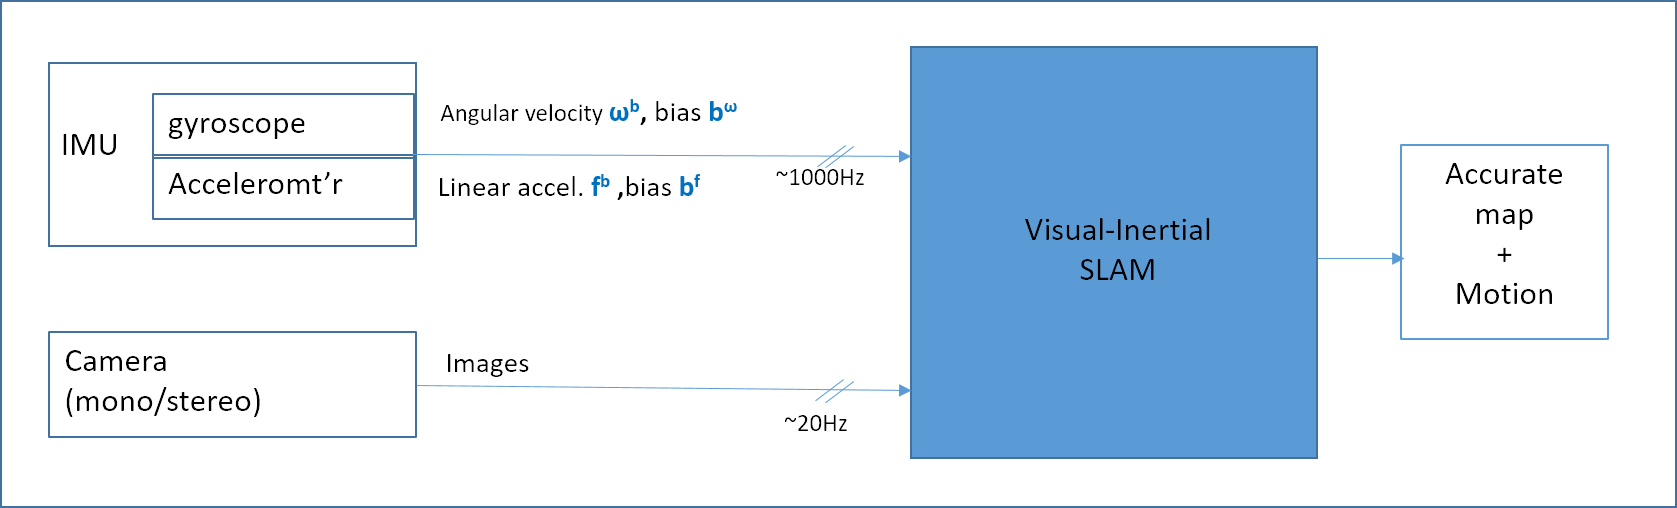
\includegraphics[height=5cm]{figures/VIN_block-diagram.png}
	\caption{Visual Inertial System}
	\label{fig:vin}
\end{figure}

\paragraph{States}
The state vector to be estimated contains the 3-D body position
$\bm{p}^{\mathrm{w}}$, velocity $\bm{v}^{\mathrm{w}}$ and rotations in form of
quaternion $\bm{q}^{\mathrm{w}}$ (converted from raw Euler angles
$\bm{A}^{\mathrm{w}}=[\alpha,\beta,\gamma]$); as well as the M feature locations
($\bm{f}_i^{\mathrm{w}}$) representing visual landmarks where i = 1,...N. 

\paragraph{IMU measurement model}
% The IMU readings include 3-D linear acceleration $\bm{f}^{\mathrm{b}}$ and
% angular rate $\bm{\omega}^{\mathrm{b}}$, both given in body frame and come
% with non-zero bias : $\bm{b}_f$ and $\bm{b}_\omega$. \newline Further, due to
% its design principal, the IMU can only measure acceleration with the gravity
% taken out, therefore the true vehicle's acceleration in the world frame should
% be \\
% $\bm{f}^{\mathrm{w}} = R_b^{\mathrm{w}}( \bm{f}^{\mathrm{b}}-\bm{b}_f ) +
% \bm{g}^{\mathrm{w}}$ \\
For the notation of coordinate transformation and vectors, superscript refers to
the reference frame and here $\{\cdot\}^{\mathrm{w}}$ is the
reference(\textbf{world}) frame. $R_b^{\mathrm{w}}$ and $\Omega_b^{\mathrm{w}}$
are the rotation and angular rate matrices from body frame to world frame,
respectively.


\begin{equation}
	\left\{
	\begin{aligned}
	&\hat{\bm{a}}^b=\bm{a}^b+\bm{b}_a+\bm{R}_w^b\bm{g}^w+\bm{n}_a\\
	&\hat{\bm{\omega}}^b=\bm{\omega}^b+\bm{b}_\omega+\bm{n}_\omega
	\end{aligned}
	\right.
	\label{eq.measurement_model}
\end{equation}
where $\hat{\bm{a}}^b$ and $\hat{\bm{\omega}}^b$ represent the measured
acceleration and angular velocity information of IMU; $\bm{a}^b$ and
$\bm{\omega}^b$ represent true acceleration and angular velocity of the body
itself; $\bm{b}_a$ and $\bm{b}_\omega$ represent the bias of the accelerator and
gyroscope, modeled as the random walk process:
\begin{equation}
\centering
	\left\{
	\begin{aligned}
	&\bm{n}_{\bm{b}_a}\sim\mathcal{N}\left(\bm{0},\bm{\sigma}_{b_a}^2\right),\bm{n}_{\bm{b}_\omega}\sim\mathcal{N}\left(\bm{0},\bm{\sigma}_{b_\omega}^2\right)\\
	&\dot{\bm{b}_a}=\bm{n}_{\bm{b}_a},dot{\bm{b}_\omega}=\bm{n}_{\bm{b}_\omega}
	\end{aligned}
	\right.
	\label{eq.error_model}
\end{equation}
where $\bm{R}_w^b$ is the coordinate rotation matrix from world coordinate to
ego-body coordinate; $\bm{g}^w$ is the gravity acceleration vector under world
coordinate; $\bm{n}_a\sim\mathcal{N}\left(\bm{0},\bm{\sigma}_a^2\right)$ and
$\bm{n}_\omega\sim\left(\bm{0},\bm{\sigma}_\omega^2\right)$ are the Gaussian
white noise of the IMU sensor.
	

\paragraph{Naive visual inertial model}

The motion model based on IMU reading can be stated as
\begin{align}
\begin{split}
	\textrm{time difference:}  \qquad \triangle t & =  t_{t+1} - t_t \\
	\textrm{acceleration:} 	   \qquad \bm{a}_t^{\mathrm{w}} & = R_{bt}^{\mathrm{w}}  (\bm{a}_t^{\mathrm{b}} - \bm{b}_a) \\
	\textrm{velocity:}         \qquad \quad \bm{v}_{t+1} & = \bm{v}_{t} + \bm{a}_t^{\mathrm{w}} \triangle t + \bm{g}^{\mathrm{w}} \triangle t \\
	\textrm{position:}         \qquad \quad \bm{p}_{t+1} & = \bm{p}_{t} + \bm{v}_t \triangle t + \bm{a}_t^{\mathrm{w}} \triangle t^2\\
	\textrm{rotation:}         \qquad \quad \bm{q}_{t+1} & = \bm{q}_t \otimes  \Omega_{bt}^{\mathrm{w}}  (\hat{\bm{\omega}}^b_t - \bm{b}_\omega) \triangle t
\end{split}
\label{eq.motion_model}
\end{align}

\chapter{Measurement Preprocessing}

\section{The original IMU problem}
For a system composed of an IMU and stereo camera navigating with $N$ camera
poses, $K$ IMU samples per image and $M$ features, the naive VI problem includes
robot poses at all IMU sample times.

\paragraph{State Vector}
the state vector $\textbf{X}$ is defined as:
\begin{align*}
\textbf{x} = &(\overbrace{\textbf{q}_{10}, \textbf{p}_{10}, \textbf{q}_{20}, \textbf{p}_{20},... ,\textbf{p}_{K-1,0}, \textbf{p}_{K-1,0},\textbf{q}_{0,1}, \textbf{p}_{0,1},...,\textbf{q}_{K-1,1}, \textbf{p}_{K-1,1},... \textbf{q}_{K-1,N-1}, \textbf{p}_{K-1,N-1},\textbf{q}_{0N}, \textbf{p}_{0N}}^{K \times (N - 1) \ {\mathrm{ poses}}},\\
	 &\overbrace{\textbf{F}_{1},\textbf{F}_{2}, ..., \textbf{F}_{M}}^{M \ {\mathrm{ features}}},\\
	 &\overbrace{\textbf{v}_{00},\textbf{v}_{10} ...,\textbf{v}_{K-1,0}, ...,\textbf{v}_{0,N-1},...,\textbf{v}_{K-1,N-1}, \textbf{v}_{0N}}^{(K \times (N-1)+1)  \ {\mathrm{ velocities}}},\\
	 &\textbf{g}^{\mathrm{n}}, \textbf{A}_{u2c}, \textbf{T}_{u2c}, \textbf{b}_f, \textbf{b}_w )^{\mathrm{T}} 
	 \label{eq.state_vector}
\end{align*}

\paragraph{Observation Vector}
The Observation vector $\textbf{Z}$ is defined as:

\begin{align*}
\begin{split}
\textbf{z}_{raw} &= (\textbf{z}_{camera}, \textbf{z}_{IMUraw}, \textbf{z}_{Tv})' \nonumber \\
=& (\overbrace{\textbf{uv}_{11}, \textbf{uv}_{21}, ... , \textbf{uv}_{M1}, ..., \textbf{uv}_{1N}, \textbf{uv}_{2N}, ... , \textbf{uv}_{MN}}^{M \times N \ {\mathrm{pixels}}}, \nonumber \\ 
& \overbrace{\omega\textbf{f}_{01}, \omega\textbf{f}_{11}, ... , \omega\textbf{f}_{(K-1)1}, ..., \omega\textbf{f}_{0(N-1)}, \omega\textbf{f}_{1(N-1)}, ... , \omega\textbf{f}_{(K-1)(N-1)}}^{K \times (N-1) \ {\mathrm{IMU \ readings}}}, \\
& \overbrace{\textbf{0}, \textbf{0}, ... , \textbf{0}}^{K \times (N-1)  \ {\mathrm{ zero \ contraints}}})^{\mathrm{T}}
\end{split}
% \label{eq.observation_vector}
\end{align*}

% See Appendix \ref{apn:naiveVin} for details on Naive VI motion model and
% optimization details. 
Clearly, such a large state space quickly becomes difficult to manage in
practice. Further, each step of re-linearization, the integration from
acceleration to velocity then to position has to be recomputed, which brings
lots of additional time.

\subsection{The Preintegration algorithm}

\begin{figure}[!h]
	\begin{center}\begin{tabular}{cc}
		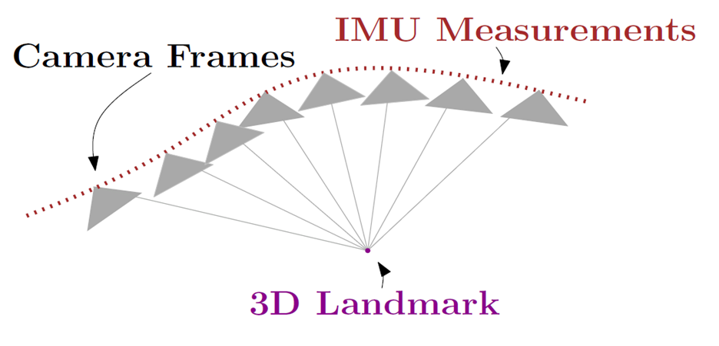
\includegraphics[height=3.3cm]{figures/IMU-sample_Image-frames_3D_illustration.png}&
		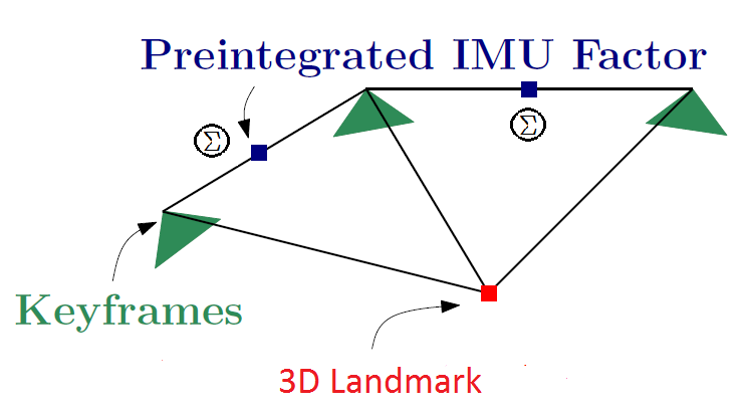
\includegraphics[height=3.3cm]{figures/Preintegrated-IMU_image_3D_illustration.png}\\
		(a) & (b) \\
	\end{tabular}\end{center}
	\caption{(a) Camera+IMU (b) Inertial-delta: preintegrated information \cite{Manifold2015}} 
	\label{fig:VIN sensor information}
\end{figure} 

Todd Lupton first proposed the Preintegration method in 2012 \cite{Lupton2012}:
integrate a large number of high rate IMU observations into a single
observation, making it faster and easier to deal with in a SLAM filter. IMU data
is integrated in a body fixed frame that moves with the vehicle, transformation
to reference frame only happens at the end of integration, hence the algorithm
is referred to as \textbf{Pre-Integration}.

The reference frame in Preintegration visual inertial system is defined as the
body frame at initial robot pose, instead of the traditional globally referenced
frame, preventing the need to reintegrate the state dynamics at each
optimization step.

%With a stereo camera, Todd Lupton also provided a way to recover the absolute
%global frame after 3 images of observation. However this is not possible with
%monocular camera setup.
\section{Formulation of Preintegration}\label{sec:preintegration}
For time consecutive frames $b_k$ and $b_{k+1}$, there exists several
measurements in the time interval $[t_k, t_{k+1}]$. Given the bias estimation,
we integrate them in the \textbf{local frame} $b_K$ as:

\begin{equation}
\centering
\left\{
\begin{aligned}
&\bm{p}_{b_{k+1}}^{b_k}=\iint_{t\in\left[t_k,t_{k+1}\right]}\bm{R}_{t}^{b_k}\left(\hat{\bm{a}}_{t}-\bm{b}_{a_t}\right)dt^2\\
&\bm{v}_{b_{k+1}}^{b_k}=\int_{t\in\left[t_k,t_{k+1}\right]}\bm{R}_{t}^{b_k}\left(\hat{\bm{a}}_{t}-\bm{b}_{a_t}\right)dt \\
&\bm{q}_{b_{k+1}}^{b_k}=\int_{t\in\left[t_k,t_{k+1}\right]}\frac{1}{2}\bm{\Omega}\left(\hat{\bm{\omega}}_t-\bm{b}_{\omega_t}\right)\bm{q}_t^{b_k}dt
\end{aligned}
\right.
\label{eq.preintegration}
\end{equation}
where $\bm{p}$, $\bm{v}$ and $\bm{q}$ are respectively the
incremental preintegration items for position, velocity and rotation (quaternion
form). Here 

\begin{equation}
\bm{\Omega}\left( \omega \right) = 
\begin{bmatrix}
	- \lfloor \omega \rfloor _ \times & \omega \\
	- \omega ^{\mathrm{T}} & 0
\end{bmatrix}, \lfloor \omega \rfloor _ \times = 
\begin{bmatrix}
	0 & - \omega_z & \omega_y \\
	- \omega_z & 0 & - \omega_x \\
	- \omega_y & \omega_x & 0
\end{bmatrix}.
\label{eq.rot_incremental}
\end{equation}

The details can be found in Appendix (\textcolor{red}{TODO}).


\subsection{Bias Correctioin of Incremental preintegration (Continuous Form)}

If the estimation of bias changes minorly, we adjust $\bm{p}_{b_{k+1}}^{b_k}$, $\bm{v}_{b_{k+1}}^{b_k}$, and $\bm{q}_{b_{k+1}}^{b_k}$ by their first-order approximations with respect to the bias as

\begin{equation}
\left\{
\begin{aligned}
&\bm{p}_{b_{k+1}}^{b_k}\approx\hat{\bm{p}}_{b_{k+1}}^{b_k}+\bm{J}^{\bm{p}}_{\bm{b}_{ak}}\delta\bm{b}_a+\bm{J}^{\bm{p}}_{\bm{b}_\omega}\delta\bm{b}_{\omega_k} \\
&\bm{v}_{b_{k+1}}^{b_k}\approx\hat{\bm{v}}_{b_{k+1}}^{b_k}+\bm{J}^{\bm{v}}_{\bm{b}_{ak}}\delta\bm{b}_a+\bm{J}^{\bm{v}}_{\bm{b}_\omega}\delta\bm{b}_{\omega_k} \\
&\bm{q}_{b_{k+1}}^{b_k}\approx\hat{\bm{q}}_{b_{k+1}}^{b_k}\otimes 
	\begin{bmatrix}
		1 \\ \frac{1}{2}\bm{J}^{\bm{q}}_{\bm{b}_{\omega_k}}\delta\bm{b}_{\omega_k}
	\end{bmatrix}.
%\bm{J}^{\bm{q}}_{\bm{b}_{\omega_k}}\delta\bm{b}_{\omega_k}
\end{aligned}
\right.
\label{eq.bias_correction}
\end{equation}

Otherwise if the estimation of bias changes significantly, which far away from the linearization point, we have to do re-propagation under the new bias estimation. So we do not have to propagate IMU measurements repeatedly which save a lot of computational resources.

% \begin{algorithm}
% 	\caption{The Pre-integration Method Based on Inertial Raw Data}
% 	\label{algm:preint}		
% 	\begin{algorithmic}
% 	\STATE Inertial-delta observation $ \triangle \bm{\mathrm{I}} =
% 		\begin{bmatrix} \triangle \textbf{p}_{t}^+ \\ \triangle \textbf{v}_{t}
% 		\\ \triangle \textbf{A} _{t} \end{bmatrix}$, initially set to
% 		$\begin{bmatrix} 0 \\ 0 \\ 0 \end{bmatrix}$ \FOR{$t_1 < t < t_2$} \STATE
% 		$\triangle t =  t_{t+1} - t_t$ \STATE $\textbf{f}_t^{\mathrm{bt1}} =
% 		R_{\mathrm{bt}}^{\mathrm{bt1}} (\textbf{f}_t^{\mathrm{b}} -
% 		\textbf{b}_f)$ \STATE $\triangle \textbf{v}_{t+1} = \triangle
% 		\textbf{v}_{t} + \textbf{f}_t^{\mathrm{bt1}} \triangle t$ \STATE
% 		$\triangle \textbf{p}_{t+1}^+ = \triangle \textbf{p}_{t}^+ + \triangle
% 		\textbf{v}_t \triangle t$ \STATE $\triangle \textbf{A} _{t+1} =
% 		\triangle \textbf{A} _{t} + E_{\mathrm{bt}}^{\mathrm{bt1}} (\omega
% 		_t^{\mathrm{b}} - \textbf{b}_\omega) \triangle t$ \ENDFOR
% 	\end{algorithmic}
% \end{algorithm}


\subsection{Bias Correctioin of Incremental preintegration (Continuous Form)}

In the code, we actually use the discrete form of preintegration using mean value method to deploy the preintegration, 
which corresponds to "IntegrationBase" in the code.

\begin{equation}
	\left\{
	\begin{aligned}
	&\bm{p}_{b_{k+1}}^{b_k}\approx\hat{\bm{p}}_{b_{k+1}}^{b_k}+\bm{v}_{b_{k+1}}^{b_k}\delta\bm{b}_a+\bm{J}^{\bm{p}}_{\bm{b}_\omega}\delta\bm{b}_{\omega_k} \\
	&\bm{v}_{b_{k+1}}^{b_k}\approx\hat{\bm{v}}_{b_{k+1}}^{b_k}+\bm{J}^{\bm{v}}_{\bm{b}_{ak}}\delta\bm{b}_a+\bm{J}^{\bm{v}}_{\bm{b}_\omega}\delta\bm{b}_{\omega_k} \\
	&\bm{q}_{b_{k+1}}^{b_k}\approx\hat{\bm{q}}_{b_{k+1}}^{b_k}\otimes 
		\begin{bmatrix}
			1 \\ \frac{1}{2}\bm{J}^{\bm{q}}_{\bm{b}_{\omega_k}}\delta\bm{b}_{\omega_k}
		\end{bmatrix}.
	%\bm{J}^{\bm{q}}_{\bm{b}_{\omega_k}}\delta\bm{b}_{\omega_k}
	\end{aligned}
	\right.
	\label{eq.discrete}
	\end{equation}

\chapter{System Initialization}


As we are using stereo cameras, we don't need to estimate an unknown metric scale factor. The initialization can be simplified into two parts: (1) Vision only SFM (Structure from Motion) (2) Alignment of vision and IMU.

\section{Vision-only SFM}

\begin{itemize}
	\item Solve the relative pose using essential matrix.
	\item Triangulate the key points to get the depth and 3D position.
	\item Solve the pose using PnP method.
	\item Coordinate transformation.
	
\end{itemize}


\section{Alignment of Vision and IMU}

Check the code in "VisualIMUAlignment"

\begin{itemize}
	\item Gyroscope bias calibration.
	\item Vlocity, Gravity vector initialization.
	\item Gravity refinement.
	\item Completing initialization.
	
\end{itemize}

Set the rotation matrix between two camera frames $\bm{R}_{c_k}^{c_{k+1}}$, the orientation matrix of IMU is $\bm{R}_{b_k}^{b_{k+1}}$ obtained by IMU pre-integration), and the extrinsic calibration between camera and IMU is $\bm{R}_b^c$, then for any two adjacent frames, we have:

\begin{equation}
	\bm{R}_{b_k}^{b_{k+1}}\bm{R}_b^c = \bm{R}_b^c\bm{R}_{c_k}^{c_{k+1}}
\end{equation}

Similarly, the orientation matrix of INS can be directly read as $\bm{R}_{w}^{b_{k+1}}$, the rotation from $k+1$ frame w.r.t. ENU coordinate, denoted as $w$. So we can obtain the rotation matrix to the absolute origin.

\begin{equation}
\bm{R}_{w}^{c_{k+1}} = \bm{R}_{w}^{b_{k+1}}\bm{R}_b^c
\end{equation}





\chapter{Backend Optimization}

We utilize the "tightly coupled" optimization framework for the final pose output. The idea is to construct a joint optimization problem by putting the residuals of vision observations and IMU/GPS/INS observations to obtain a global optimal result.

To constraint the number of optimization variables, we use sliding window method with the state variables:

%\begin{equation}
%	\begin{aligned}
%		\mathcal{X} &= \left[  \mathbf{x}_0, \mathbf{x}_0, \cdots, \mathbf{x}_n, \mathbf{x}_c^b, \lambda_0, \lambda_1, \cdots, \lambda_m  \right] \\
%		\mathbf{x}_k &= \left[  \mathbf{x}_{b_k}^w, \mathbf{v}_{b_k}^w, \mathbf{q}_{b_k}^w, \mathbf{v}_a, \mathbf{v_g}  \right], k\in{[0, n]} \\
%		\mathbf{x}_c^b &= \left[ \mathbf{p}_c^b, \mathbf{q}_c^b \right]
%	\end{aligned}
%\end{equation}

\begin{equation}
\begin{aligned}
\mathbf{\mathcal{X}} &= \left[  \mathbf{x}_0, \mathbf{x}_0, \cdots, \mathbf{x}_n, \lambda_0, \lambda_1, \cdots, \lambda_m  \right] \\
\mathbf{x}_k &= \left[  \mathbf{x}_{b_k}^w, \mathbf{v}_{b_k}^w, \mathbf{q}_{b_k}^w  \right], k\in{[0, n]} 
%\mathbf{x}_c^b &= \left[ \mathbf{p}_c^b, \mathbf{q}_c^b \right]
\end{aligned} \label{states}
\end{equation}

where $\mathbf{x}_k$ represents all the camera states inside the sliding window containing $n+1$ keyframes (including positions, rotations, and velocities); $\mathbf{\lambda}_k$ is inverse depth of $m+1$ 3D points~\ref{civera2008inverse}.

Additionally for IMU sensor, the states $\mathbf{x}_k$ also contain biases of gyroscope and accelerator $\mathbf{b}_g$ and $\mathbf{b}_a$.


Here we list the parametrization of map points defined in the code:

\begin{cppcode}
class FeaturePerId {
//Index of this map point.
const int feature_id;
// The frame index of first observation of this map point.
int start_frame;
// Vector of features in each frame(observation). 
// Its size is the number of observations.
vector<FeaturePerFrame> feature_per_frame;
// Size of @ref feature\_per\_frame, observation times.
int used_num;
// Estimated depth in meters.
double estimated_depth;
// Flag of depth estimation successful or not.
// 0 haven't solve yet; 1 solve succ; 2 solve fail (estimated depth <0);
int solve_flag;
};
\end{cppcode}


So the cost function for minimizing the residuals from all sensors can be formulated as a bundle adjustment problem:

\begin{equation}
	\min_{\mathcal{X}}  \left\{
		\underbrace{
			\left\|\mathbf{r}_{p}-\mathbf{H}_{p} \mathcal{X}\right\|^{2}
		}_{\text{Marginalization Priors}}
		+
		\underbrace{
			\sum_{k \in \mathcal{B}}\left\|\mathbf{r}_{\mathcal{B}}\left(\hat{\mathbf{z}}_{b_{k+1}}^{b_{k}}, \mathcal{X}\right)\right\|_{\mathbf{P}_{b_{k}+1}^{2}}^{2}
		}_{\text{IMU/INS Factors}}
		+
		\underbrace{
			\sum_{(l, j) \in \mathcal{C}} \rho\left(\left\|\mathbf{r}_{\mathcal{C}}\left(\hat{\mathbf{z}}_{l}^{c_{j}}, \mathcal{X}\right)\right\|_{\mathbf{P}_{l}^{c_{j}}}^{2}\right)
		}_{\text{Vision Factors}}
		\right\} \label{joint_optimization}
\end{equation}

Note that:
\begin{itemize}
	\item All the residuals represent Mahalanobis distance by dividing the scalar measurements with standard deviation (this process is called \textit{whitening} to eliminate the metrics \cite{dellaert2017factor}).
	\item We use Huber loss function as the robust kernel function $\rho(\cdot)$ to tackle visual outliers.
\end{itemize}


\section{Vision Factors}


\subsection{Residuals}

	Vision factors are \textbf{reprojection error of feature points}. The visual residuals together with their Jacobian matrix calculation can be referred to in \verb|ProjectionFactor::Evaluate| function. 
	
	For the key point in the $i$th frame, we can get the projection location under the camera coordinate of the $j$th frame.
	
\begin{equation}
	\left[\begin{array}{c}
	{x_{c_{j}}} \\ {y_{c_{j}}} \\ {z_{c_{j}}} \\ {1}
	\end{array}\right] =
	\mathbf{T}_{b c}^{-1} 
	\mathbf{T}_{w b_{j}}^{-1} 
	\mathbf{T}_{w b_{i}} 
	\mathbf{T}_{b c}
	\left[\begin{array}{c}
	{\frac{1}{\lambda} u_{c_{i}}} \\ 
	{\frac{1}{\lambda} v_{c_{i}}} \\ 
	{\frac{1}{\lambda}} \\ 
	{1}
	\end{array}\right]\label{reproj_error}
\end{equation}
where $u_{c_i}$ and $v_{c_i}$ are the image pixel location of $ith$ frame with inverse depth $\lambda$; $\mathbf{T}_{b c}$ is the transformation matrix ($4\times4$) from camera to IMU, $\mathbf{T}_{w b_{i}}$ is the transformation matrix from from $ith$ IMU frame to ENU coordinate.
	
	So its 3D position can be represented as:
	
\begin{equation}
	\label{equ:pcj}
	\begin{aligned} 
	\mathbf{P}_{c_{j}} 
	&=
	\left[\begin{array}{c}
	{x_{c_{j}}} \\ {y_{c_{j}}} \\ {z_{c_{j}}}
	\end{array}\right] 
	=
	\mathbf{R}_{b c}^{\top} \left(
	\mathbf{R}_{w b_{j}}^{\top} \left(
	\mathbf{R}_{w b_{i}} \left(
	\mathbf{R}_{b c} 
	\mathbf{P}_{c_i}
	+ \mathbf{p}_{b c} \right)
	+ \mathbf{p}_{w b_{i}} - \mathbf{p}_{w b_{j}}\right)
	- \mathbf{p}_{b c}\right) \\
	&=
	\mathbf{R}_{b c}^{\top} 
	\mathbf{R}_{w b_{j}}^{\top} 
	\mathbf{R}_{w b_{i}} 
	\mathbf{R}_{b c} 
	\mathbf{P}_{c_i} +
	\mathbf{R}_{b c}^{\top}
	\left(\mathbf{R}_{w b_{j}}^{\top} 
	\left(\left(\mathbf{R}_{w b_{i}} \mathbf{p}_{b c}+\mathbf{p}_{w b_{i}}\right)
	-\mathbf{p}_{w b_{j}}\right)-\mathbf{p}_{b c}\right) 
	\end{aligned}
\end{equation}
	
where 

\begin{equation}
	\label{equ:pci}
	\mathbf{P}_{c_i} = \frac{\bar{\mathbf{P}}_{c_{i}}}{\lambda} = 
	\frac{1}{\lambda}
	\left[\begin{array}{c}
	{u_{c_{i}}} \\ {v_{c_{i}}} \\ {1}
	\end{array}\right]
\end{equation}
	
For the convenience of calculating Jacobian, we disassemble equation\ref{equ:pcj} and define the following variables:

\begin{equation}
\label{equ:f_predef}
\begin{array}{l}
{\mathbf{f}_{b_{i}}=\mathbf{R}_{b c} \mathbf{P}_{c_{i}}+\mathbf{p}_{b c}} \\ {\mathbf{f}_{w}=\mathbf{R}_{w b_{i}} \mathbf{f}_{b_{i}}+\mathbf{p}_{w b_{i}}} \\ {\mathbf{f}_{b_{j}}=\mathbf{R}_{w b_{j}}^{\top}\left(\mathbf{f}_{w}-\mathbf{p}_{w b_{j}}\right)} \\
{\mathbf{P}_{c_{j}}=\mathbf{R}_{b c}^{\top}\left(\mathbf{f}_{b_{j}}-\mathbf{p}_{b c}\right)}
\end{array}
\end{equation}

\begin{cppcode}
// Convert the 3D point under frame i to the frame j coordinate.
Eigen::Vector3d pts_camera_i = pts_i / inv_dep_i;
Eigen::Vector3d pts_imu_i    = qic * pts_camera_i + tic;
Eigen::Vector3d pts_w        = Qi * pts_imu_i + Pi;     
Eigen::Vector3d pts_imu_j    = Qj.inverse() * (pts_w - Pj); 
Eigen::Vector3d pts_camera_j = qic.inverse() * (pts_imu_j - tic);
\end{cppcode}

So the vision residuals are:

\begin{equation}
\label{equ:residual_visual}
\mathbf{r}_{c} =
\Sigma \cdot
\left[\begin{array}{c}
{\frac{x_{c_{j}}}{z_{c_{j}}}-u_{c_{j}}} \\ 
{\frac{y_{c_{j}}}{z_{c_{j}}}-v_{c_{j}}}
\end{array}\right] =
\Sigma \cdot
\left(\frac{P_{c_{j}}}{Z_j} - \hat{\bar{P}}_{c_{j}}\right)_2
\in \mathbb{R}^{2 \times 1}
\end{equation}


\begin{cppcode}
Eigen::Map<Eigen::Vector2d> residual(residuals);
residual =  tangent_base * (pts_camera_j.normalized() - pts_j.normalized());
// Get the error on the normalized plane.
double dep_j = pts_camera_j.z();
residual = (pts_camera_j / dep_j).head<2>() - pts_j.head<2>();
// transform Euclidean distance to Mahalanobis distance
residual = sqrt_info * residual; 
\end{cppcode}


\subsection{Covariance Matrix}

We set a fixed covariance matrix by setting the image standard deviation as $1.5$ pixels.

\begin{equation}
\Sigma = 
\begin{bmatrix}
\frac{f}{1.5} & 0 \\
0 & \frac{f}{1.5}
\end{bmatrix}
\end{equation}

\begin{cppcode}
ProjectionFactor::sqrt_info = FOCAL_LENGTH / 1.5 * Matrix2d::Identity();
\end{cppcode}


\subsection{Jacobian Matrix}

Jacobian matrix is defined as the derivatives of visual residuals to the states and reverse depth values of two time stamps.

\begin{equation}
\mathbf{J} = 
\frac{\partial \mathbf{r}_{c}}{\partial \mathbf{X}_{c}} =
\begin{bmatrix}
\frac{\partial \mathbf{P}_{c_{j}}}
{\partial\left[\begin{array}{c}{\delta \mathbf{p}_{w b_{i}}} \\ 
	{\delta \boldsymbol{\theta}_{w b_{i}}}\end{array}\right]} 
&
\frac{\partial \mathbf{P}_{c_{j}}}
{\partial\left[\begin{array}{c}{\delta \mathbf{p}_{w b_{j}}} \\ 
	{\delta \boldsymbol{\theta}_{w b_{j}}}\end{array}\right]} 
&
\frac{\partial \mathbf{P}_{c_{j}}}
{\partial\left[\begin{array}{c}{\delta \mathbf{p}_{bc}} \\ 
	{\delta \boldsymbol{\theta}_{bc}}\end{array}\right]} 
&
\frac{\partial \mathbf{P}_{c_{j}}}{\partial \delta \lambda}
\end{bmatrix} \label{jacobian}
\end{equation}

According to the chain rule, we have

\begin{equation}
\begin{aligned}
\mathbf{J} 
&= 
\frac{\partial \mathbf{r}_{c}}{\partial \mathbf{P}_{c_{j}}}
\frac{\partial \mathbf{P}_{c_{j}}}{\partial \mathbf{X}_{c}}
=
\mathbf{J}_1 \mathbf{J}_2 \\
&=
\frac{\partial \mathbf{r}_{c}}{\partial \mathbf{P}_{c_{j}}}
\begin{bmatrix}
\frac{\partial \mathbf{P}_{c_{j}}}
{\partial\left[\begin{array}{c}{\delta \mathbf{p}_{w b_{i}}} \\ 
	{\delta \boldsymbol{\theta}_{w b_{i}}}\end{array}\right]} 
&
\frac{\partial \mathbf{P}_{c_{j}}}
{\partial\left[\begin{array}{c}{\delta \mathbf{p}_{w b_{j}}} \\ 
	{\delta \boldsymbol{\theta}_{w b_{j}}}\end{array}\right]} 
&
\frac{\partial \mathbf{P}_{c_{j}}}
{\partial\left[\begin{array}{c}{\delta \mathbf{p}_{bc}} \\ 
	{\delta \boldsymbol{\theta}_{bc}}\end{array}\right]} 
&
\frac{\partial \mathbf{P}_{c_{j}}}{\partial \delta \lambda}
\end{bmatrix}
\end{aligned}
\end{equation}


For the first part $\mathbf{J}_1$, according to equation\eqref{equ:residual_visual}:

\begin{equation}
\mathbf{J}_1 =
\frac{\partial \mathbf{r}_{c}}{\partial \mathbf{P}_{c_{j}}} = 
\Sigma \cdot
\left[\begin{array}{ccc}
{\frac{1}{z_{c_{j}}}} & {0} & {-\frac{x_{c_{j}}}{z_{c_{j}}^{2}}} \\ 
{0} & {\frac{1}{z_{c_{j}}}} & {-\frac{y_{c_{j}}^{2}}{z_{c_{j}}^{2}}}
\end{array}\right]
\in \mathbb{R}^{2 \times 3}
\end{equation}

\begin{cppcode}
Eigen::Matrix<double, 2, 3> reduce(2, 3);
reduce << 1. / dep_j, 0, -pts_camera_j(0) / (dep_j * dep_j),
0, 1. / dep_j, -pts_camera_j(1) / (dep_j * dep_j);
reduce = sqrt_info * reduce;
\end{cppcode}


Then for the second part $\mathbf{J}_2$, according to equation\eqref{equ:pcj}\eqref{equ:pci}\eqref{equ:f_predef}, we get the partial derivatives of different state variables:

\begin{enumerate}
	
	\item[(a)] Partial derivatives of {\color{blue} state variables $[\delta p^{w}_{b_{i}},\delta \theta ^{w}_{b_{i}}]$ at $i$ th timestamp}

	
	\begin{equation}
	\begin{aligned}
	\frac{\partial \mathbf{P}_{c_{j}}}{\partial \delta \mathbf{p}_{w b_{i}}} 
	&=
	\mathbf{R}_{b c}^{\top} \mathbf{R}_{w b_{j}}^{\top} 
	\\
	\frac{\partial \mathbf{P}_{c_{j}}}{\partial \delta \boldsymbol{\theta}_{w b_{i}}} 
	&=
	\frac{\partial \mathbf{R}_{b c}^{\top} \mathbf{R}_{w b_{j}}^{\top} \mathbf{R}_{w b_{i}}\left(\mathbf{I}+\left[\delta \boldsymbol{\theta}_{wb_{i}}\right]_{\times}\right) \mathbf{f}_{b_{i}}}{\partial \delta \boldsymbol{\theta}_{wb_{i}}} 
	\quad \text{(Abandon irrelavent parts)} \\
	&=
	-\mathbf{R}_{b c}^{\top} \mathbf{R}_{w b_{j}}^{\top} \mathbf{R}_{w b_{i}}\left[\mathbf{f}_{b_{i}}\right]_{\times}
	\end{aligned}
	\end{equation}
	
	\begin{equation}
	\mathbf{J}_2[0] 
	=
	\frac{\partial \mathbf{P}_{c_{j}}}
	{\partial \left[\begin{array}{c}{\delta \mathbf{p}_{w b_{i}}} \\ 
		{\delta \boldsymbol{\theta}_{w b_{i}}}\end{array}\right]} 
	=
	\begin{bmatrix}
	\mathbf{R}_{b c}^{\top} \mathbf{R}_{w b_{j}}^{\top} & 
	-\mathbf{R}_{b c}^{\top} \mathbf{R}_{w b_{j}}^{\top} \mathbf{R}_{w b_{i}}\left[\mathbf{f}_{b_{i}}\right]_{\times}
	\end{bmatrix}
	\in \mathbb{R}^{3 \times 6}
	\end{equation}
	
	\item[(b)] Partial derivatives of {\color{blue} state variables $[\delta p^{w}_{b_{j}},\delta \theta ^{w}_{b_{j}}]$ at $j$ timestamp}
	
	\begin{equation}
	\begin{aligned}
	\frac{\partial \mathbf{P}_{c_{j}}}{\partial \delta \mathbf{p}_{w b_{j}}} 
	&=
	-\mathbf{R}_{b c}^{\top} \mathbf{R}_{w b_{j}}^{\top} 
	\\
	\frac{\partial \mathbf{P}_{c_{j}}}{\partial \delta \boldsymbol{\theta}_{w b_{j}}} 
	&=
	\frac{\partial \mathbf{R}_{b c}^{\top}\left(\mathbf{I}-\left[\delta \boldsymbol{\theta}_{w b_{j}}\right]_{\times}\right) \mathbf{R}_{w b_{j}}^{\top}\left(\mathbf{f}_{w}-\mathbf{p}_{w b_{j}}\right)}
	{\partial \delta \boldsymbol{\theta}_{w b_{j}}} \\
	&=
	\frac{\partial \mathbf{R}_{b c}^{\top}\left(\mathbf{I}-\left[\delta \boldsymbol{\theta}_{w b_{j}}\right]_{\times}\right) \mathbf{f}_{b_{j}}}
	{\partial \delta \boldsymbol{\theta}_{w b_{j}}} \\
	&=
	\mathbf{R}_{b c}^{\top}\left[\mathbf{f}_{b_{j}}\right]_{\times}
	\end{aligned}
	\end{equation}
	
	\begin{equation}
	\mathbf{J}_2[1]
	=
	\frac{\partial \mathbf{P}_{c_{j}}}
	{\partial \left[\begin{array}{c}{\delta \mathbf{p}_{w b_{j}}} \\ 
		{\delta \boldsymbol{\theta}_{w b_{j}}}\end{array}\right]} 
	=
	\begin{bmatrix}
	-\mathbf{R}_{b c}^{\top} \mathbf{R}_{w b_{j}}^{\top} 
	& 
	\mathbf{R}_{b c}^{\top}\left[\mathbf{f}_{b_{j}}\right]_{\times}
	\end{bmatrix}
	\in \mathbb{R}^{3 \times 6}
	\end{equation}
	
	\item[(c)] Partial derivatives of {\color{blue} extrinsic parameters between IMU and cameras $[\delta p^{b}_{c},\delta \theta ^{b}_{c}]$} (Optional)
	
	\begin{equation}
	\begin{aligned}
	\frac{\partial \mathbf{P}_{c_{j}}}{\partial \delta \mathbf{p}_{bc}} 
	={}& 
	\mathbf{R}_{b c}^{\top}\left(\mathbf{R}_{w b_{j}}^{\top} \mathbf{R}_{w b_{i}}-\mathbf{I}_{3 \times 3}\right) 
	\\
	\frac{\partial \mathbf{P}_{c_{j}}}{\partial \delta \boldsymbol{\theta}_{bc}} 
	={}&
	\frac{\partial 
		\mathbf{R}_{b c}^{\top} 
		\mathbf{R}_{w b_{j}}^{\top} 
		\mathbf{R}_{w b_{i}} 
		\mathbf{R}_{b c} 
		\mathbf{P}_{c_i}}
	{\partial \delta \boldsymbol{\theta}_{bc}} 
	+
	\frac{\partial 
		\mathbf{R}_{b c}^{\top}
		\left(\mathbf{R}_{w b_{j}}^{\top} 
		\left(\left(\mathbf{R}_{w b_{i}} \mathbf{p}_{b c}+\mathbf{p}_{w b_{i}}\right)
		-\mathbf{p}_{w b_{j}}\right)-\mathbf{p}_{b c}\right)}
	{\partial \delta \boldsymbol{\theta}_{bc}} \\
	={}&
	\frac{\partial 
		\left(\mathbf{I}-\left[\delta \boldsymbol{\theta}_{bc}\right]_{\times}\right)
		\mathbf{R}_{b c}^{\top} 
		\mathbf{R}_{w b_{j}}^{\top} 
		\mathbf{R}_{w b_{i}} 
		\mathbf{R}_{b c} 
		\left(\mathbf{I}+\left[\delta \boldsymbol{\theta}_{bc}\right]_{\times}\right)
		\mathbf{P}_{c_i}}
	{\partial \delta \boldsymbol{\theta}_{bc}} \\
	&+
	\frac{\partial 
		\left(\mathbf{I}-\left[\delta \boldsymbol{\theta}_{bc}\right]_{\times}\right)
		\mathbf{R}_{b c}^{\top}
		\left(\mathbf{R}_{w b_{j}}^{\top} 
		\left(\left(\mathbf{R}_{w b_{i}} \mathbf{p}_{b c}+\mathbf{p}_{w b_{i}}\right)
		-\mathbf{p}_{w b_{j}}\right)-\mathbf{p}_{b c}\right)}
	{\partial \delta \boldsymbol{\theta}_{bc}} \\
	={}&
	\left(-\mathbf{R}_{b c}^{\top} \mathbf{R}_{w b_{j}}^{\top} \mathbf{R}_{w b_{i}} \mathbf{R}_{b c}\left[\mathbf{P}_{c_{i}}\right]_{\times} + \left[\mathbf{R}_{b c}^{\top} \mathbf{R}_{w b_{j}}^{\top} \mathbf{R}_{w b_{i}} \mathbf{R}_{b c} \mathbf{P}_{c_{i}}\right]_{\times}\right) \\
	&+
	\left[\mathbf{R}_{b c}^{\top}\left(\mathbf{R}_{w b_{j}}^{\top}\left(\left(\mathbf{R}_{w b_{i}} \mathbf{p}_{b c}+\mathbf{p}_{w b_{i}}\right)-\mathbf{p}_{w b_{j}}\right)-\mathbf{p}_{b c}\right)\right]_{\times}
	\end{aligned}
	\end{equation}
	
	\begin{equation}
	\mathbf{J}_2[2] =
	\frac{\partial \mathbf{P}_{c_{j}}}
	{\partial\left[\begin{array}{c}{\delta \mathbf{p}_{bc}} \\ 
		{\delta \boldsymbol{\theta}_{bc}}\end{array}\right]} =
	\begin{bmatrix}
	\frac{\partial \mathbf{P}_{c_{j}}}{\partial \delta \mathbf{p}_{bc}} &
	\frac{\partial \mathbf{P}_{c_{j}}}{\partial \delta \boldsymbol{\theta}_{bc}} 
	\end{bmatrix}
	\in \mathbb{R}^{3 \times 6}
	\end{equation}
	
	\item[(d)] Partial derivatives of {\color{blue}feature point inverse depth $\delta \lambda$}
	
	\begin{equation}
	\begin{aligned} 
	\frac{\partial \mathbf{P}_{c_{j}}}{\partial \delta \lambda} 
	&=
	\frac{\partial \mathbf{P}_{c_{j}}}{\partial \mathbf{P}_{c_{i}}} 
	\frac{\partial \mathbf{P}_{c_{i}}}{\partial \delta \lambda} \\ 
	&=
	\mathbf{R}_{b c}^{\top} \mathbf{R}_{w b_{j}}^{\top} \mathbf{R}_{w b_{i}} \mathbf{R}_{b c}
	\left(-\frac{1}{\lambda^{2}}
	\left[\begin{array}{c}{u_{c_{i}}} \\ {v_{c_{i}}} \\ {1}\end{array}\right]\right) \\ 
	&=
	-\frac{1}{\lambda} \mathbf{R}_{b c}^{\top} \mathbf{R}_{w b_{j}}^{\top} \mathbf{R}_{w b_{i}} \mathbf{R}_{b c} \mathbf{P}_{c_{i}} 
	\end{aligned}
	\end{equation}
	
	\begin{equation}
	\mathbf{J}_2[3] =
	\frac{\partial \mathbf{P}_{c_{j}}}{\partial \delta \lambda}
	\in \mathbb{R}^{3 \times 1}
	\end{equation}
	
\end{enumerate}


All the above codes can be seen in \verb|factor/projectionXFrameXCamFactor.cpp|.

\section{IMU Factor}

This section is quite complicated. 

\subsection{Residuals}

According to the explanation of IMU pre-integration in section~\ref{sec:preintegration}, we acquire the pre-integration residuals:

\begin{equation}
\label{equ:residual_imu_origin}
\mathbf{r}_{\mathcal{B}}\left(\hat{\mathbf{z}}_{b_{k+1}}^{b_{k}}, \mathcal{X}\right) 
=
\left[\begin{array}{c}
{\delta \boldsymbol{\alpha}_{b_{k+1}}^{b_{k}}} \\ 
{\delta \boldsymbol{\theta}_{b_{k+1}}^{b_{k}}} \\
{\delta \boldsymbol{\beta}_{b_{k+1}}^{b_{k}}} \\ 
{\delta \mathbf{b}_{b_{k}}} \\ 
{\delta \mathbf{b}_{g_{k}}}
\end{array}\right]_{15 \times 1} 
= 
\left[\begin{array}{c}
{\mathbf{R}_{w}^{b_{k}}
	\left(\mathbf{p}_{b_{k+1}}^{w}-\mathbf{p}_{b_{k}}^{w}+\frac{1}{2} \mathbf{g}^{w} \Delta t_{k}^{2}-\mathbf{v}_{b_{k}}^{w} \Delta t_{k}\right)-
	\color{blue}{\boldsymbol{\alpha}_{b_{k+1}}^{b_{k}}}} \\ 
{2\left[\mathbf{q}_{b_{k}}^{w^{-1}} \otimes \mathbf{q}_{b_{k+1}}^{w} \otimes\left({\color{blue}{{\gamma}_{b_{k+1}}^{b_{k}}}}\right)^{-1}\right]_{x y z}} \\
{\mathbf{R}_{w}^{b_{k}}\left(\mathbf{v}_{b_{k+1}}^{w}+\mathbf{g}^{w} \Delta t_{k}-\mathbf{v}_{b_{k}}^{w}\right) - \color{blue}{\boldsymbol{\beta}}_{b_{k+1}}^{b_{k}}} \\  
{\mathbf{b}_{a b_{k+1}}-\mathbf{b}_{a b_{k}}} \\ 
{\mathbf{b}_{w b_{k+1}}-\mathbf{b}_{w b_{k}}}
\end{array}\right]
\end{equation}

where $[\color{blue}{{\alpha}^{b_{k}}_{b_{k+1}},{\gamma}^{b_{k}}_{b_{k+1}},{\beta}^{b_{k}}_{b_{k+1}}}]$ is the bias correction value.

Rewrite the above equation \eqref{equ:residual_imu_origin} into quaternion form:

\begin{equation}
\label{equ:residual_imu_q}
\mathbf{r}_{\mathcal{B}}
=
\left[\begin{array}{c}
{\mathbf{r}_{p}} \\ 
{\mathbf{r}_{q}} \\ 
{\mathbf{r}_{v}} \\ 
{\mathbf{r}_{b a}} \\ 
{\mathbf{r}_{b g}}
\end{array}\right]
=
\left[\begin{array}{c}
{\mathbf{q}_{b_{i} w}\left(\mathbf{p}_{w b_{j}}-\mathbf{p}_{w b_{i}}-\mathbf{v}_{i}^{w} \Delta t+\frac{1}{2} \mathbf{g}^{w} \Delta t^{2}\right)-{\color{blue}\boldsymbol{\alpha}_{b_{i} b_{j}}}} \\ 
{2\left[{\color{blue}\mathbf{q}_{b_{j} b_{i}}} \otimes\left(\mathbf{q}_{b_{i} w} \otimes \mathbf{q}_{w b_{j}}\right)\right]_{xyz}} \\ 
{\mathbf{q}_{b_{i} w}\left(\mathbf{v}_{j}^{w}-\mathbf{v}_{i}^{w}+\mathbf{g}^{w} \Delta t\right)-{\color{blue}\boldsymbol{\beta}_{b_{i} b_{j}}}} \\ 
{\mathbf{b}_{j}^{a}-\mathbf{b}_{i}^{a}} \\ 
{\mathbf{b}_{j}^{g}-\mathbf{b}_{i}^{g}}
\end{array}\right]_{15 \times 1}
\end{equation}

\begin{cppcode}
Eigen::Quaterniond dq_rected = delta_q * Utility::deltaQ(dq_dbg * dbg);
Eigen::Vector3d    dv_rected = delta_v + dv_dba * dba + dv_dbg * dbg;
Eigen::Vector3d    dp_rected = delta_p + dp_dba * dba + dp_dbg * dbg;

residuals.block<3, 1>(O_P, 0)  = 
Qi.inverse() * (0.5*G*sum_dt*sum_dt + Pj - Pi - Vi*sum_dt) - dp_rected;
residuals.block<3, 1>(O_R, 0)  = 
2 * (dq_rected.inverse() * (Qi.inverse() * Qj)).vec();
residuals.block<3, 1>(O_V, 0)  = 
Qi.inverse() * (G * sum_dt + Vj - Vi) - dv_rected;
residuals.block<3, 1>(O_BA, 0) = Baj - Bai;
residuals.block<3, 1>(O_BG, 0) = Bgj - Bgi;
\end{cppcode}

\subsection{Covariance Matrix}

The covariance matrix $\boldsymbol{\Sigma}$ is the $\mathbf{P}$ calculated from the previous IMU pre-integration. 

\begin{cppcode}
Eigen::Map<Eigen::Matrix<double, 15, 1>> residual(residuals);
residual=pre_integration->evaluate(Pi, Qi, Vi, Bai, Bgi, Pj, Qj, Vj, Baj, Bgj);

Eigen::Matrix<double, 15, 15> cov_inv = pre_integration->covariance.inverse();
Eigen::Matrix<double, 15, 15> sqrt_info =
Eigen::LLT<Eigen::Matrix<double, 15, 15>>(cov_inv).matrixL().transpose();

residual = sqrt_info * residual; 
\end{cppcode}

Once we get the covariance (\verb|sqrt_info|), we use that to calculate the Mahalanobis distance by multiplying with \verb|residual|

\begin{equation}
\|\mathbf{r}\|^2_{\boldsymbol{\Sigma}} = \mathbf{r}^T \boldsymbol{\Sigma}^{-1} \mathbf{r}
\end{equation}

\subsection{Jacobian Matrix}

We still need to calculate the partial derivatives of error state variables according to equation \eqref{equ:residual_imu_q}.

\begin{enumerate}
	\item Partial derivatives to {\color{blue} $[\delta p^{w}_{b_{i}},\delta \theta ^{w}_{b_{i}}]$} at $ith$ frame.
	\begin{equation}
	\mathbf{J}[0]=
	\begin{bmatrix}
	-\mathbf{R}_{b_{i} w} & \left[\mathbf{R}_{b_{i} w}\left(\mathbf{p}_{w b_{j}}-\mathbf{p}_{w b_{i}}-\mathbf{v}_{i}^{w} \Delta t+\frac{1}{2} \mathbf{g}^{w} \Delta t^{2}\right)\right]_{\times} \\
	\mathbf{0} & -2\left[\begin{array}{ll}{\mathbf{0}} & {\mathbf{I}}\end{array}\right]\left[\mathbf{q}_{w b_{j}}^{*} \otimes \mathbf{q}_{w b_{i}}\right]_{L}\left[\mathbf{q}_{b_{i} b_{j}}\right]_{R}\left[\begin{array}{c}{\mathbf{0}} \\ {\frac{1}{2} \mathbf{I}}\end{array}\right] \\
	\mathbf{0} & \left[\mathbf{R}_{b_{i} w}\left(\mathbf{v}_{j}^{w}-\mathbf{v}_{i}^{w}+\mathbf{g}^{w} \Delta t\right)\right]_{\times} \\
	\mathbf{0} & \mathbf{0}  \\
	\mathbf{0} & \mathbf{0} 
	\end{bmatrix}
	\in \mathbb{R}^{15 \times 7}
	\end{equation}
	
	\item Partial derivatives to {\color{blue}$[\delta v^{w}_{i},\delta b^a_{i},\delta b^g_{i}]$} at $ith$ frame.
	
	\begin{equation}
	\mathbf{J}[1]=
	\begin{bmatrix}
	-\mathbf{R}_{b_{i} w} \Delta t & -\mathbf{J}_{b_{i}^{a}}^{\alpha} & -\mathbf{J}_{b_{i}^{g}}^{\alpha} \\
	\mathbf{0} & \mathbf{0} & -2\left[\begin{array}{ll}{\mathbf{0}} & {\mathbf{I}}\end{array}\right]\left[\mathbf{q}_{w b_{j}}^{*} \otimes \mathbf{q}_{w b_{i}} \otimes \mathbf{q}_{b_{i} b_{j}}\right]_{L}\left[\begin{array}{c}{\mathbf{0}} \\ {\frac{1}{2} \mathbf{J}_{b_{i}^{g}}^{q}}\end{array}\right] \\
	-\mathbf{R}_{b_{i} w} & -\mathbf{J}_{b_{i}^{a}}^{\beta} & -\mathbf{J}_{b_{i}^{g}}^{\beta} \\
	\mathbf{0} & -\mathbf{I}  &  \mathbf{0} \\
	\mathbf{0} &  \mathbf{0}  & -\mathbf{I}
	\end{bmatrix}
	\in \mathbb{R}^{15 \times 9}
	\end{equation}
	
	\item Partial derivatives to {\color{blue}$[\delta p^{w}_{b_{j}},\delta \theta ^{w}_{b_{j}}]$} at $ith$ frame.
	
	\begin{equation}
	\mathbf{J}[2]=
	\begin{bmatrix}
	\mathbf{R}_{b_{i} w} & \mathbf{0} \\
	\mathbf{0} & 2\left[\begin{array}{ll}{\mathbf{0}} & {\mathbf{I}}\end{array}\right]\left[\mathbf{q}_{b_{i} b_{j}}^{*} \otimes \mathbf{q}_{w b_{i}}^{*} \otimes \mathbf{q}_{w b_{j}}\right]_{L}\left[\begin{array}{c}{\mathbf{0}} \\ {\frac{1}{2} \mathbf{I}}\end{array}\right] \\
	\mathbf{0} & \mathbf{0} \\
	\mathbf{0} & \mathbf{0}  \\
	\mathbf{0} & \mathbf{0}   
	\end{bmatrix}
	\in \mathbb{R}^{15 \times 7}
	\end{equation}
	
	\item Partial derivatives to {\color{blue}$[\delta v^{w}_{j},\delta b^a_{j},\delta b^g_{j}]$} at $ith$ frame.
	
	\begin{equation}
	\mathbf{J}[3]=
	\begin{bmatrix}
	\mathbf{0} & \mathbf{0} & \mathbf{0} \\
	\mathbf{0} & \mathbf{0} & \mathbf{0} \\
	\mathbf{R}_{b_{i} w} & \mathbf{0} & \mathbf{0} \\
	\mathbf{0} & \mathbf{I} & \mathbf{0} \\
	\mathbf{0} & \mathbf{0} & \mathbf{I}
	\end{bmatrix}
	\in \mathbb{R}^{15 \times 9}
	\end{equation}
	
\end{enumerate}



\section{INS Factor}




\section{GPS Factor}






\section{Marginalization}

\begin{figure}[htbp]
	\centering
	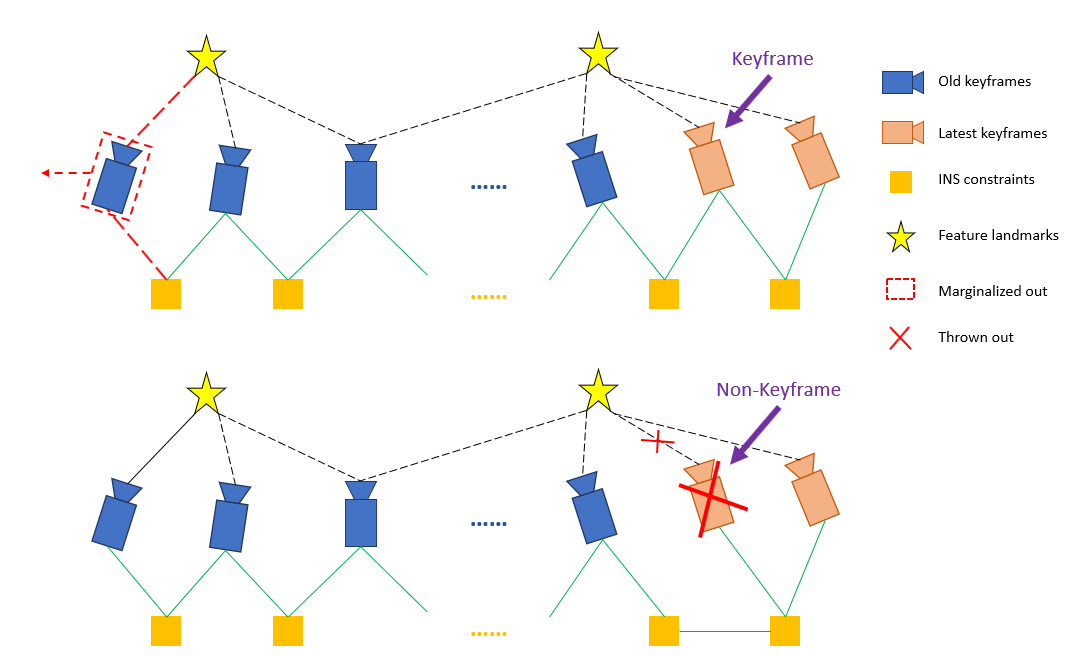
\includegraphics[scale=0.5]{figures/marginalization.png}
\end{figure}

Sliding window constraints the number of key-frames to keep a bound of finite complexity by restraining the accumulating of pose and feature numbers with time going on.

\subsection{Marginalization Concept}

When we are using sliding window, we have to abandon old poses, thus culling out some constraints, which is bound to cause the decrease of accuracy. So instead of directly "throwing out" the constraints, it is better converting the related constraints into a prior constraint in the optimization called "marginalization".

The process of marginalization is the process of \textbf{decomposing joint probability distribution into marginal probability distribution and conditional probability distribution}, also can be taken as the reduction of parameters to be optimized using Shur Complement algorithm.


It is known that there exists sparsity in the Hessian matrix in the visual SLAM case according to the optimization theory. For example, a residual only describes the error that at camera pose $\mathbf{x}_i$ we observed landmark $\mathbf{p}_j$, so the Jacobian matrix of this residual contains all 0 values except the $\mathbf{x}_i$ and $\mathbf{p}_j$ entries. Hessian matrix is the quadratic form of Jacobian: $\mathbf{H} = \mathbf{J}^T\mathbf{T}$. 



So for the Hessian matrix we can decompose it into four blocks by converting the equation $\mathbf{p}_j$ into:

\begin{equation}
\label{eq:linearequations}
\left[ \begin{matrix}
\bm{B}   &   \bm{E} \\
\bm{E^\mathrm{T}} &   \bm{C}
\end{matrix}\right] 
\left[ \begin{array}{l}
\Delta \bm{x}_c \\
\Delta \bm{x}_p 
\end{array} \right] = 
\left[ \begin{array}{l}
\bm{v} \\
\bm{w} 
\end{array} \right].
\end{equation}

where $\bm{B}$ is a diagonal matrix with dimension of each diagonal block the same as camera parameter and the number of diagonal blocks the same as camera variable numbers. As each landmark we only record the inverse depth value, so the dimension of each block is $1\times1$. 




The use of marginalization is very popular among key-frame based SLAM methods. It is used in \textit{g2o} for calculation speedup by eliminating landmark variables first and then try to solve camera pose first to in turn solve the landmark variables. While in our system, we need to really marginalize out the oldest or last new frames to maintain their relationships with the current sliding window without the need to calculate them.








\begin{equation}\label{eq:guasselimination}
\left[ \begin{matrix}
\bm{I}   &    -\bm{EC^{-1}} \\
\bm{0}	 &	  \bm{I}
\end{matrix}\right]
\left[ \begin{matrix}
\bm{B}   &   \bm{E} \\
\bm{E^\mathrm{T}} &   \bm{C}
\end{matrix}\right] 
\left[ \begin{array}{l}
\Delta \bm{x}_c \\
\Delta \bm{x}_p 
\end{array} \right] = 
\left[ \begin{matrix}
\bm{I}   &    -\bm{EC^{-1}}  \\
\bm{0}	 &	  \bm{I}
\end{matrix}
\right]
\left[ \begin{array}{l}
\bm{v} \\
\bm{w} 
\end{array} \right]  .
\end{equation}

Then we get:

\begin{equation}
\left[ \begin{matrix}
\bm{B} - \bm{E}\bm{C}^{-1}\bm{E}^\mathrm{T}	& 	\bm{0} \\
\bm{E}^\mathrm{T}							& 	\bm{C}
\end{matrix} \right]
\left[ \begin{array}{l}
\Delta \bm{x}_c \\
\Delta \bm{x}_p 
\end{array} \right] = 
\left[\begin{array}{l}
\bm{v} - \bm{E}\bm{C}^{-1}\bm{w}  \\
\bm{w}
\end{array}\right].
\label{mid_schur}
\end{equation}

where $\bm{E}\bm{C}^{-1}\bm{E}^\mathrm{T}$ is called the \textbf{Schur factor} of $\bm{C}$ in $\bm{E}$. After elimination, the first line becomes irrelevant with $\Delta \bm{x}_p$. So we extract it and get the incremental equation of the "pose" part.

\begin{equation}
\left[ 
\bm{B} - \bm{E}\bm{C}^{-1}\bm{E}^\mathrm{T}
\right]
\Delta \bm{x}_c  = 
\bm{v} - \bm{E}\bm{C}^{-1}\bm{w}.
\label{eq:marginalization}
\end{equation}

The dimension of this linear equation is the same as $\bm{B}$ matrix. So we first solve the equation and replace the solved $\Delta \bm{x}_c$ into the original equation and get $\Delta \bm{x}_p$. This process is called \textcolor{blue}{Schur Elimination}. 


\subsection{Toy Example of Marginalization}

The process of marginalization and the follow-up phenomenon called "fill-in" (the Hessian matrix becomes dense) can be illustrated in this section. 

Suppose we have 4 camera poses $\bm{x}_{pi}$ and 6 landmarks $\bm{x}_{mk}$, the links between camera and landmarks represent a visual observation and the links between camera poses are INS/IMU constraints. Then we can get:


\begin{figure}[H]
	\centering
	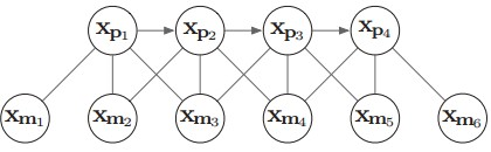
\includegraphics[width=.6\linewidth]{figures/before_marg.png}
	\caption{Graph relationships of 4 camera poses observing 6 landmarks.}
	\label{fig:before_marg}
\end{figure}

Then if we try to marginalize out $\bm{x}_{p1}$, and then marginalize out $\bm{x}_{m1}$, the change of Hessian matrix $\bm{H}$ is illustrated as:

\begin{figure}[H]
	\centering
	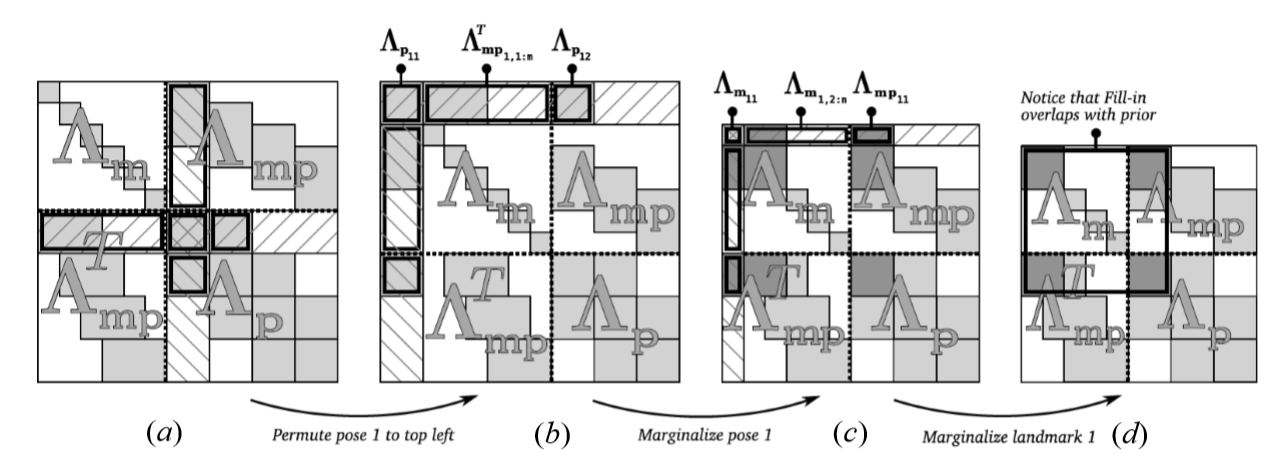
\includegraphics[width=1.0\linewidth]{figures/marg_process_fillin.png}
	\caption{The change of $\bm{H}$ matrix when marginalizing out pose and landmark.}
	\label{fig:marg_process_fillin}
\end{figure}

To explain this in details, let \ref{fig:marg_process_fillin}-(a) represent the original $\bm{H}$ matrix with the top-left part landmark related information and bottom-right part pose information. \ref{fig:marg_process_fillin}-(b) moves the part related to $\bm{x}_{p1}$ to the top left corner of the $\bm{H}$ matrix.

\ref{fig:marg_process_fillin}-(c) is the matrix after marginalizing out the $\bm{x}_{p1}$ values, which represents the $\left( \bm{B} - \bm{E}\bm{C}^{-1}\bm{E}^\mathrm{T} \right)$ in equation \eqref{eq:marginalization}. As you can see, compared to (b), \ref{fig:marg_process_fillin}-(c) becomes denser (the color becomes darker) by filling-in three places.

\begin{figure}[H]
	\centering
	\begin{subfigure}[t]{.4\linewidth}
	\centering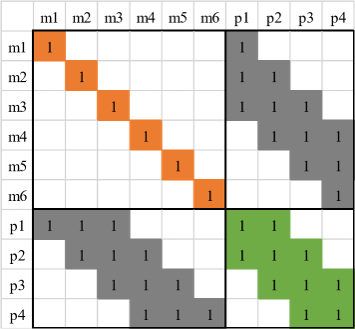
\includegraphics[width=.8\linewidth]{figures/marg_01.png}
	\caption{Representation of \ref{fig:marg_process_fillin}-a.}
	\end{subfigure}
	\begin{subfigure}[t]{.4\linewidth}
		\centering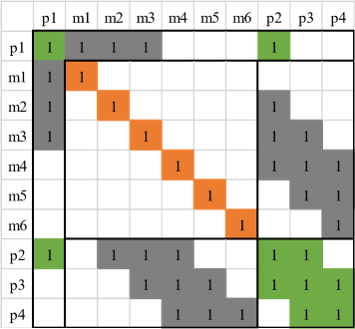
\includegraphics[width=.8\linewidth]{figures/marg_02.png}
		\caption{Representation of \ref{fig:marg_process_fillin}-b.}
	\end{subfigure}
	\begin{subfigure}[t]{.4\linewidth}
	\centering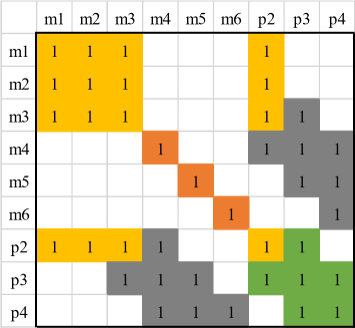
\includegraphics[width=.8\linewidth]{figures/marg_03.png}
	\caption{Representation of \ref{fig:marg_process_fillin}-a.}
\end{subfigure}
\begin{subfigure}[t]{.4\linewidth}
	\centering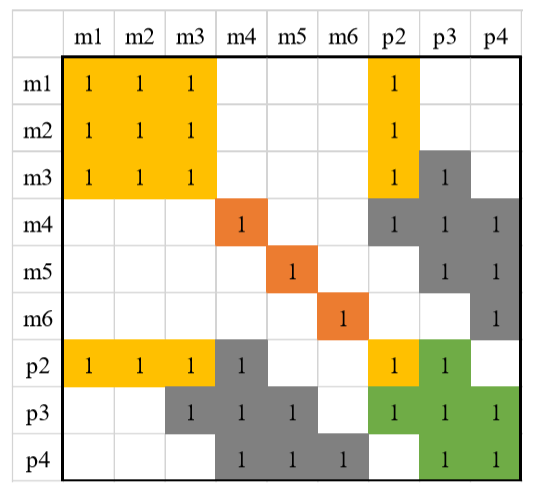
\includegraphics[width=.8\linewidth]{figures/marg_04.png}
	\caption{Representation of \ref{fig:marg_process_fillin}-b.}
\end{subfigure}
\caption{Detailed illustration of Hessian matrix during marginalization.}
\end{figure}

At this time, the new graph becomes:


\begin{figure}[H]
	\centering
	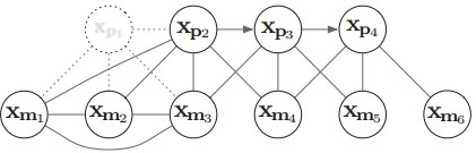
\includegraphics[width=.6\linewidth]{figures/after_marg.png}
	\caption{Graph relationships after marginalizing out $\bm{x}_{p1}$.}
	\label{fig:after_marg}
\end{figure}

As you can see there exist new constraints between $\bm{x}_{m1}$, $\bm{x}_{m2}$ and $\bm{x}_{m3}$, and also between $\bm{x}_{p2}$ and $\bm{x}_{m1}$.

If you further marginalize out $\bm{x}_{m1}$, actually $\bm{H}$ does not become denser as seen in \ref{fig:marg_process_fillin}-(d). That's because $\bm{x}_{m1}$ does not relate to other poses except $\bm{x}_{p1}$. So marginalizing out landmarks not observed by other frames will not make the $\bm{H}$ matrix denser. 



\subsection{Implementation}


We first define the marginalization factor in \textit{Ceres} according to the dimension of different variables to be optimized.

\begin{cppcode}
struct ResidualBlockInfo{
ceres::CostFunction *_cost_function, 
ceres::LossFunction *_loss_function,
// Variable values to be optimized.
std::vector<double *> _parameter_blocks, 
// Variable values to be marginalized out.
std::vector<int> _drop_set}

\end{cppcode}


\begin{cppcode}
class MarginalizationInfo {
// (1) All the observable factors (in form of residual block information).
std::vector<ResidualBlockInfo *> factors;
// (2) pos: size of all variables (local size).
// (3) n: number of remaining variables to be optimized (local size).
// (4) m: number of variables to be marginalized (local size).
int m, n;

// "parameter\_block\_sizes":
// parameters in cost\_function is an array of pointers to arrays
// csame number of elements as parameter\_block\_sizes.  
// Parameter blocks are in the same order as parameter\_block\_sizes. i.e.,
//   parameters\_[i] = double[parameter\_block\_sizes\_[i]]

// (5) The memory address of variables to be optimized.
// <long, int> where first element is address of variable.
// second element is the number of outputs (residuals)
std::unordered_map<long, int> parameter_block_size;
// (6) Corresponding data (double*) of "parameter\_block\_size".
std::unordered_map<long, double *> parameter_block_data;
int sum_block_size;
// Ids in "parameter\_block\_size", the memory address
// of variables to be marginalized.
std::unordered_map<long, int> parameter_block_idx; //local size

std::vector<int> keep_block_size; //global size
std::vector<int> keep_block_idx;  //local size
std::vector<double *> keep_block_data;
Eigen::MatrixXd linearized_jacobians;
Eigen::VectorXd linearized_residuals;
// Add residual block information (all variables to be optimized).
void addResidualBlockInfo(ResidualBlockInfo *residual_block_info);

// Calculate Jacobian of each residual, and update "parameter\_block\_data"
void preMarginalize();

// pos: dimension of all variables.
void marginalize();
}
\end{cppcode}

\begin{itemize}
	\item \verb|parmaeter_block_data|	\\
	 When the oldest keyframe is to be marginalized, the term \verb|parameter_block_size| is the local size of all variables and  \verb|parameter_block_data| is the corresponding stored data (double* type). 
	Set the oldest frame (namely $0th$ frame) the camera observed $k=68$ landmarks, then the size of both \verb|parameter_block_size| and \verb|parameter_block_data| vector is:
	
	\begin{equation*}
	2(V_0, V_1) + 11(P_{0:10}) + 68(\lambda_{1:k}) = 81
	\end{equation*}
	
	Considering the variable dimension, the total local size of all variables is:
	
	\begin{equation*}
	pos = 2\times 9 + 11\times 6 + 68 = 152
	\end{equation*}
	
	\item \verb|parameter_block_idx| \\
	
	\verb|parameter_block_idx| is the variables that need to be marginalized. So the size of the array of \verb|parameter_block_idx| is:
	
	\begin{equation*}
	1(P_0) + 1(V_0) + 68(\lambda_{1:k}) = 70
	\end{equation*}
	
	If we use $m$ to represent the total local size of the variables to be marginalized, (namely $m=6+9+68=83$), then we use $n$ to indicate the total local size of the variable to be kept: $n=pos-m = 152-83=69$.
	
\end{itemize}


Inspired by VINS~\cite{qin2017vins}, we introduce a two-way marginalization method to handle the static motion case. 

\begin{enumerate}
	\item \verb|MARGIN_OLD|: If the last new frame is a keyframe, we abandon the oldest frame in the sliding window and implement marginalization to tackle the related constraints of this old frame. It is worth noting that, if this keyframe is the first frame to observe some 3D map point, we need to convert the depth of this map point to the next keyframe.
	
	\begin{enumerate}
		\item Transmit the residual item (size is $n$) of last prior factor to the current prior facotr and remove the states to be abandoned.
		\item If there is IMU pre-integration items (when there is IMU sensor input), we put the IMU constraint between the $0th$ and $1th$ frame into the \verb|marginalization_info| class.
		\item For the landmark points that were observed for the first time at the $0th$ frame, we put them into the \verb|marginalization_info| class.
		\item \verb|marginalization_info->preMarginalize()|: Calculate the \verb|parameter_blocks| and the corresponding jacobians and residuals before formulating the optimization problem.
		\item \verb|marginalization_info->marginalize()|: Calculate the equation \eqref{eq:marginalization}.
		
\begin{cppcode}
// Line 301 in sslam\_estimator/src/factor/
// marginalization\_factor.cpp. 
Eigen::VectorXd bmm = b.segment(0, m);
Eigen::MatrixXd Amr = A.block(0, m, m, n);
Eigen::MatrixXd Arm = A.block(m, 0, n, m);
Eigen::MatrixXd Arr = A.block(m, m, n, n);
Eigen::VectorXd brr = b.segment(m, n);
A = Arr - Arm * Amm_inv * Amr;
b = brr - Arm * Amm_inv * bmm;
\end{cppcode}
		
	\end{enumerate}
	
	
	\item \verb|MARGIN_NEW|: If the last new frame is not a keyframe, then abandon it without the need of marginalization. Since our strategy of judging whether a frame is a keyframe is that it has low parallax with the previous frame, we can directly replace the current frame with the last new frame. The similar constraints will not bring additional effective information so we can directly delete that frame without losing accuracy. 
	
\end{enumerate}

So if the UGV stays in the same location for a long time, the VO system will always implement \verb|MARGIN_NEW| and the sliding window will only keep the poses that are relative "old" but with a big parallax. In this way we can reduce the accumulating drift cost by camera and INS/IMU small errors.




















\newpage 
%-----------------------------------------------------------------------------------------
%----------------------------------------------------------------------------------------
%	BIBLIOGRAPHY
%----------------------------------------------------------------------------------------
%\chapter{Bibliography}
%\label{Bibliography}

\bibliographystyle{plainnat}
\bibliography{vins} % The references (bibliography) information are stored in


\end{document}

